\documentclass[12pt]{article}

\usepackage{listings}
\usepackage{cite}
\usepackage{graphicx}
\usepackage{booktabs}
\usepackage{color}
\usepackage{indentfirst}
\usepackage{multirow}
\usepackage{url}
\usepackage{setspace}

\definecolor{codegreen}{rgb}{0,0.6,0}
\definecolor{codegray}{rgb}{0.5,0.5,0.5}
\definecolor{codepurple}{rgb}{0.58,0,0.82}
\definecolor{backcolour}{rgb}{0.95,0.95,0.92}
\definecolor{codeblue}{rgb}{0.7,0.8,0.215}

\lstdefinestyle{newStyle}{
    backgroundcolor=\color{backcolour},   
    commentstyle=\color{codegreen},
    keywordstyle=\color{blue},
    numberstyle=\tiny\color{codegray},
    stringstyle=\color{codepurple},
    basicstyle=\footnotesize,
    breakatwhitespace=false,         
    breaklines=true,                 
    captionpos=b,                    
    keepspaces=true,                 
    numbers=left,                    
    numbersep=5pt,                  
    showspaces=false,                
    showstringspaces=false,
    showtabs=false,                  
    tabsize=2
}
 
\lstset{style=newstyle}
\setcounter{section}{-1}
\usepackage[left=2cm,right=2cm,
    top=2cm,bottom=2cm,bindingoffset=0cm]{geometry}

\title{DESCRIPTIVE-STATISTICS}
\date{SUMMER 2018}     
 % Alphabetical order
\author{
Amandeep Kaur Khosa\\
Dmitry Kryukov\\
Kritika Kritika\\
Mehak Jot Kaur\\
Roopamdeep Kaur\\
Sukhmeet Kaur
}
%\setcounter{secnumdepth}{0}
\newcommand\tabularhead[1]{
\begin{table}[h]
  \caption{Use case - #1}
  \begin{tabular}{|p{0.35\linewidth}|p{0.65\linewidth}|}
    \hline
    \textbf{Use case name} & \textbf{#1} \\
    \hline}

  \newcommand\addrow[2]{#1 &#2\\ \hline}
  
  \newcommand\adddoublerow[2]{\begin{minipage}[t][][t]{2.5cm}#1\end{minipage}%
    &\begin{minipage}[t][][t]{\linewidth}
     \begin{itemize}\setlength{\itemsep}{0pt}%
        #2     
     \end{itemize}
     \end{minipage}\\ \hline}
  
  \newcommand\addmulrow[2]{ \begin{minipage}[t][][t]{2.5cm}#1\end{minipage}% 
     &\begin{minipage}[t][][t]{\linewidth}
      \begin{enumerate}\setlength{\itemsep}{0pt}%
        #2   
      \end{enumerate}
      \end{minipage}\\ \hline}
      
  \newenvironment{usecase}{\tabularhead}
{\hline\end{tabular}\end{table}}
% start of the document
\begin{document}            
%\maketitle               
%\begin{center}
%\begin{tabular}{l r}
%Instructor: & Professor PANKAJ KAMTHAN
%\end{tabular}
%\end{center}
%-----------------------------------------------------------------
\begin{titlepage}
\newcommand{\HRule}{\rule{\linewidth}{0.5mm}} 

\includegraphics[width=8cm]{clogo.jpeg}\\[1cm]
\center
\textsc{\huge Team F}\\[1.0cm]
\textsc{\LARGE Deliverable 1}\\[0.5cm]
\textsc{\Large SOEN 6611 Software Measurement}\\[0.5cm]
\textsc{\large Department of Software Engineering and Computer Science, Concordia University}\\[0.5cm]
\makeatletter

\HRule \\[1.0cm]
{ \huge \bfseries \@title}\\[0.5cm]
\HRule \\[1.5cm]

\begin{minipage}{0.4\textwidth}
\begin{flushleft} \large
\emph{Authors:}\\
\@author % Your name
\end{flushleft}
\end{minipage}
~
\begin{minipage}{0.4\textwidth}
\begin{flushright} \large
\emph{Instructor:} \\
Prof. PANKAJ KAMTHAN \\[1.2em] % Supervisor's Name
\end{flushright}
\end{minipage}\\[2cm]
\makeatother
{\large SUMMER 2018}\\[2cm] 
\vfill
\end{titlepage}
%-----------------------------------------------------------------
\newpage
\tableofcontents
%-----------------------------------------------------------------
\section{Introduction}
The purpose of the descriptive-statistics is engaged with the processing of empirical data, quantitatively describe a sets of information and systematization of the data. 

The considered project is a module which should integrate to the Online Grading System and help to improve users experience by using descriptive-statistics features. For that project were implemented from scratch a several functions: Minimum, Maximum, Mode, Median, Arithmetic Mean and Standard Deviation. According to the requirements, no built-in functions were used. The new functions were written from scratch and the whole project was written by using the R language.

During development cycle the quality attributes such as efficiency, readability,  maintainability, understandability and usability were taken into account and described in code as correct as possible.

In the project GQM approach is used to achieve the goal of the project.\cite{GQM-approach} \cite{GQM} \cite{GQM-wiki} \cite{GQM-eduardo} \cite{GQM-book} \cite{GQM-book2} \cite{GQM-Bjorn}

%-----------------------------------------------------------------
\section{Part - GQM}      
\subsection{Goal}
Create a module to \textbf{improve} the \textbf{efficiency} of studying process from the point of view of \textbf{students and professors} in the context of \textbf{online grading system}. \par 
The descriptive-statistics in the module shall provide more efficient and accurate data based on new minimum, maximum, mode, median, mean and deviation functions for assigning the grades.

\subsection{Questions}

\begin{itemize}
    \item \textbf{Q1}: How many lines of code are the files on average?\\
     M1: Number of files.\\
     M2: Number of lines of code (SLOC) in the files.\\
     M3: Average number of lines of code in the files. 
    \item \textbf{Q2}: How to ensure that the descriptive-statistics functions return results in less than 2 sec? \\
     M4: Time-based unit tests
    \item \textbf{Q3}: How to ensure that the all users satisfied with the module?\\
     M5: Student survey
    \item \textbf{Q4}: What is the defect/failures density?\\
     M6: Number of failures reported by users per month\\
     M2: Number of lines of code (SLOC) in the files.\\
     M7: Number of failures per KLOC.
    \item \textbf{Q5}: How to ensure that the code is maintainable?\\
     M8: Test coverage.
    \item \textbf{Q6}: How to ensure that the code is easy to read for other developers?\\
     M9: The code corresponds to the convention (code stardard)
    \item \textbf{Q7}: How many functions covered by documentation?\\
     M10: Number of functions\\
     M11: Number of comments\\
     M12: The ratio of the number of comments to the SLOC
    \item \textbf{Q8}: How many the unit tests are performed?\\
     M13: The ratio of performed unit tests to the number of unit tests.
    \item \textbf{Q9}: How to ensure that the descriptive-statistics functions return the correct results?\\
     M8: Test coverage.\\
     M14: Number of unit tests 
    \item \textbf{Q10}: What are the bottlenecks of increasing effectiveness of the system?\\
     M15: Action runtime
    \item \textbf{Q11}: How to ensure that the module development is profitable?\\
     M16: Effort estimation\\
     M17: Cost estimation\\
     M18: Duration estimation
    \item \textbf{Q12}: How the developers are effective at finding failures?\\
     M14: Number of unit tests\\
     M6: Number of failures reported by users per month\\
     M13: The ratio of performed unit tests to the number of unit tests. 
\end{itemize}
\newpage
%-----------------------------------------------------------------
\section{Part - Use case model}
Use case model represent the interaction between actors and the system and shows the relationships between the actors and different use cases.\cite{UCM}
\begin{figure}[h]
\centering
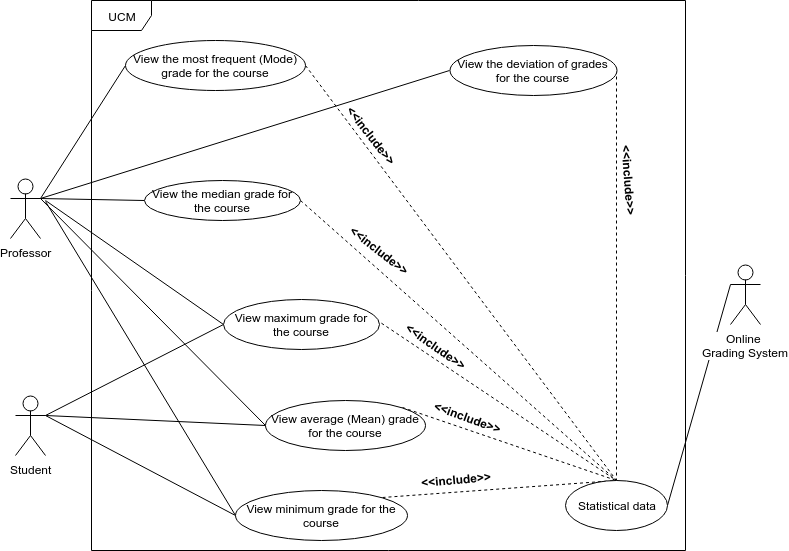
\includegraphics[width=\textwidth]{UCMv2.png}
\caption{Use case model}
\end{figure}
\newpage
\subsection{Use cases}

\begin{usecase}{View the most frequent (Mode) for the course}
    \addrow{Actors}{Professor, Online Grading System}
    \addrow{Precondition}{Professor has access to the system}
    \addrow{Postcondition}{Professor views the mode}
    \addmulrow{Main scenario (M)}{
        \item Professor logins to the system
        \item System through statistical data module connects to the Online Grading System
        \item System shows the list of available courses
        \item Professor chooses the course to view
        \item System shows the statistics of the course
        \item Professor views the mode of course
    }
    \adddoublerow{Extensions (E)}{
        \item[] 1.1. Professor entered the wrong credentials
        \item[] 1.2. Go to 1
    }
\end{usecase}

\begin{usecase}{View the deviation for the course}
    \addrow{Actors}{Professor, Online Grading System}
    \addrow{Precondition}{Professor has access to the system}
    \addrow{Postcondition}{Professor views the deviation}
    \addmulrow{Main scenario (M)}{
        \item Professor logins to the system
        \item System through statistical data module connects to the Online Grading System
        \item System shows the list of available courses
        \item Professor chooses the course to view
        \item System shows the statistics of the course
        \item Professor views the deviation for the course
    }
    \adddoublerow{Extensions (E)}{
        \item[] 1.1. Professor entered the wrong credentials
        \item[] 1.2. Go to 1
    }
\end{usecase}
\newpage
\begin{usecase}{View the median for the course}
    \addrow{Actors}{Professor, Online Grading System}
    \addrow{Precondition}{Professor has access to the system}
    \addrow{Postcondition}{Professor views the median}
    \addmulrow{Main scenario (M)}{
        \item Professor logins to the system
        \item System through statistical data module connects to the Online Grading System
        \item System shows the list of available courses
        \item Professor chooses the course to view
        \item System shows the statistics of the course
        \item Professor views the median
    }
    \adddoublerow{Extensions (E)}{
        \item[] 1.1. Professor entered the wrong credentials
        \item[] 1.2. Go to 1
    }
\end{usecase}

\begin{usecase}{View average (Mean) for the course}
    \addrow{Actors}{Professor, Student, Online Grading System}
    \addrow{Precondition}{Professor has access to the system. Student has access to the system}
    \addrow{Postcondition}{Professor views average (Mean). Student views average (Mean).}
    \addmulrow{Main scenario (M)}{
        \item Professor or Student logins to the system
        \item System through statistical data module connects to the Online Grading System
        \item System shows the list of available courses for the user (Professor or Student)
        \item Professor or Student chooses the desirable course
        \item System shows the average (Mean) for the course
    }
    \adddoublerow{Extensions (E)}{
        \item[] 1.1. Professor or Student entered the wrong credentials
        \item[] 1.2. Go to 1
    }
\end{usecase}
\newpage
\begin{usecase}{View minimum for the course}
    \addrow{Actors}{Professor, Student, Online Grading System}
    \addrow{Precondition}{Professor has access to the system. Student has access to the system}
    \addrow{Postcondition}{Professor views minimum.  Student views minimum.}
    \addmulrow{Main scenario (M)}{
        \item Professor or Student logins to the system
        \item System through statistical data module connects to the Online Grading System
        \item System shows the list of available courses for the user (Professor or Student)
        \item Professor or Student chooses the desirable course
        \item System shows the minimum for the course
    }
    \adddoublerow{Extensions (E)}{
        \item[] 1.1. Professor or Student entered the wrong credentials
        \item[] 1.2. Go to 1
    }
\end{usecase}

\begin{usecase}{View maximum for the course}
    \addrow{Actors}{Professor, Student, Online Grading System}
    \addrow{Precondition}{Professor has access to the system. Student has access to the system}
    \addrow{Postcondition}{Professor views maximum. Student views maximum .}
    \addmulrow{Main scenario (M)}{
        \item Professor or Student logins to the system
        \item System through statistical data module connects to the Online Grading System
        \item System shows the list of available courses for the user (Professor or Student)
        \item Professor or Student chooses the desirable course
        \item System shows the maximum for the course
    }
    \adddoublerow{Extensions (E)}{
        \item[] 1.1. Professor or Student entered the wrong credentials
        \item[] 1.2. Go to 1
    }
\end{usecase}
\newpage
%-----------------------------------------------------------------
\section{Part - Estimates of effort}
\subsection{UCP}
The \textbf{UCP} is effort estimation approach. To calculate effort there are number of needed equations: \textbf{UUCP} (Unadjusted Use Case Points), \textbf{TCF} (Technical Complexity Factor), \textbf{ECF} (Environment Complexity Factor). \\
\begin{equation}
    \textbf{UCP} = \textbf{UUCP} \times \textbf{TCF} \times \textbf{ECF}
\end{equation}\\

The \textbf{UUCP} based on the sum of \textbf{UAW} (Unadjusted Actor Weight)
and \textbf{UUCW} (Unadjusted Use Case Weight).\\
\begin{equation}
    \textbf{UUCP} = \textbf{UAW} + \textbf{UUCW}
\end{equation}\\

The \textbf{UAW} based on the aggregated complexity of all the actors in all the use cases.
\begin{equation}
    \textbf{UAW} = \sum^{}_{}{Actors * Weight}
\end{equation}\\
\begin{table}[h]
\centering
\begin{tabular}{|l|l|l|}
\hline
\textbf{Actor type} & \textbf{Description} & \textbf{Weight} \\ \hline
A1                  & Simple actor         & 1               \\ \hline
A2                  & Average actor        & 2               \\ \hline
A3                  & Complex actor        & 3               \\ \hline
\end{tabular}
\caption{The classification of actors and their associated weights in the UCP approach.}
\end{table}
Based on the \textbf{UCM} we have 2 complex actors and 1 simple, then:
\begin{equation}
    \textbf{UAW} = 1\times3 + 1\times3 + 1\times1
\end{equation}
\begin{equation}
    \textbf{UAW} = 7
\end{equation}\\

the \textbf{UUCW} is based on the total number of steps contained in all the use case scenarios.
\begin{equation}
    \textbf{UUCW} = \sum^{}_{}{UseCase * Weight}
\end{equation}\\
\begin{table}[h]
\centering
\begin{tabular}{|l|l|l|}
\hline
\textbf{Use Case Type} & \textbf{Description} & \textbf{Weight} \\ \hline
UC1                    & Simple Use Case      & 5               \\ \hline
UC2                    & Average Use Case     & 10              \\ \hline
UC3                    & Complex Use Case     & 15              \\ \hline
\end{tabular}
\caption{shows that there are 3 types of use cases, each assigned a weight. }
\end{table}
Based on the \textbf{UCM} we have 6 simple use cases, then:
\begin{equation}
    \textbf{UUCW} = 6 \times 5
\end{equation}
\begin{equation}
    \textbf{UUCW} = 30
\end{equation}\\

In this case the \textbf{UUCP} is:
\begin{equation}
    \textbf{UUCP} = 7 + 30
\end{equation}
\begin{equation}
    \textbf{UUCP} = 37
\end{equation}\\

The purpose of \textbf{TCF} (Technical complexity factor) is to account for the technical concerns that can impact the software project from its inception to its conclusion, including delivery.
\begin{equation}
    \textbf{TCF} = C1 + \Bigg[C2 \times \sum^{13}_{i=1}{(W_{Ti} \times F_{i})\Bigg]} 
\end{equation}\\
Where $C1 = 0.6$, $C2 = 0.01$, $W_{Ti}$ is the Technical Complexity Factor Weight, and $F_{i}$ is the Perceived Impact Factor corresponding to each Technical Complexity Factor. 

\begin{table}[h]
\centering
\begin{tabular}{|l|l|l|l|}
\hline
\multicolumn{1}{|c|}{\textbf{TCF Type}} & \multicolumn{1}{c|}{\textbf{Description}} & \multicolumn{1}{c|}{\textbf{Weight}} & \multicolumn{1}{c|}{\textbf{Factor}} \\ \hline
T1 & Distributed System & 2 & 0 \\ \hline
T2 & Performance & 1 & 5 \\ \hline
T3 & End User Efficiency & 1 & 4 \\ \hline
T4 & Complex Internal Processing & 1 & 3 \\ \hline
T5 & Reusability & 1 & 5 \\ \hline
T6 & Easy to Install & 0.5 & 4 \\ \hline
T7 & Easy to Use & 0.5 & 5 \\ \hline
T8 & Portability & 2 & 5 \\ \hline
T9 & Easy to Change & 1 & 5 \\ \hline
T10 & Concurrency & 1 & 4 \\ \hline
T11 & Special Security Features & 1 & 0 \\ \hline
T12 & Provides Direct Access for Third Parties & 1 & 0 \\ \hline
T13 & Special User Training Facilities are Required & 1 & 0 \\ \hline
\end{tabular}
\caption{The Technical Complexity Factors in the UCP approach.}
\end{table}
In this case the \textbf{TCF} is:
\begin{equation}
    \textbf{TCF} =  0.6 + \Big[0.01 \times(2\times0+1\times5+1\times4+1\times3+1\times5+0.5\times4+0.5\times5+2\times5+1\times5+1\times4+1\times0+1\times0+1\times0)\Big]
\end{equation}
\begin{equation}
    \textbf{TCF} =  1.005
\end{equation}\\
\newpage
The purpose of \textbf{ECF} is to account for the development team's personal traits, including experience.
\begin{equation}
    \textbf{ECF} = C1 + \Bigg[C2 \times \sum^{8}_{i=1}{(W_{Ei} \times F_{i})\Bigg]} 
\end{equation}\\
Where $C1 = 1.4$, $C2 = - 0.03$, $W_{Ei}$ is the Environmental Complexity Factor Weight, and $F_{i}$ is the Perceived Impact Factor corresponding to each Environmental Complexity Factor.

\begin{table}[h]
\centering
\begin{tabular}{|l|l|l|l|}
\hline
\multicolumn{1}{|c|}{\textbf{ECF Type}} & \multicolumn{1}{c|}{\textbf{Description}} & \multicolumn{1}{c|}{\textbf{Weight}} & \multicolumn{1}{c|}{\textbf{Factor}} \\ \hline
E1 & Familiarity with the Use Case Domain & 1.5 & 4 \\ \hline
E2 & Part-Time Workers & -1 & 3 \\ \hline
E3 & Analyst Capability & 0.5 & 3 \\ \hline
E4 & Application Experience & 0.5 & 4 \\ \hline
E5 & Object-Oriented Experience & 1 & 5 \\ \hline
E6 & Motivation & 1 & 5 \\ \hline
E7 & Difficult Programming Language & -1 & 5 \\ \hline
E8 & Stable Requirements & 2 & 5 \\ \hline
\end{tabular}
\caption{The Environmental Complexity Factors in the UCP approach.}
\end{table}

In this case the \textbf{ECF} is:
\begin{equation}
    \textbf{ECF} =  1.4 + \Big[-0.03 \times(1.5\times4+(-1\times3)+0.5\times3+0.5\times4+1\times5+1\times5+(-1\times5)+2\times5)\Big]
\end{equation}
\begin{equation}
    \textbf{ECF} =  0.755
\end{equation}\\

The \textbf{UCP} is equal:
\begin{equation}
    \textbf{UCP} = 37 \times 1.005 \times 0.755
\end{equation}
\begin{equation}
    \textbf{UCP} = 28.075
\end{equation}\\

Since the team is new, the \textbf{PF} (Productivity Factor) is equal \textbf{20}.
In this case the Effort Estimate is:
\begin{equation}
    \textbf{Effort Estimate} = \textbf{UCP} \times \textbf{PF}
\end{equation}
\begin{equation}
    \textbf{Effort Estimate} = 28.075 \times 20
\end{equation}
\begin{equation}
    \textbf{Effort Estimate} = 561.5 \quad \textrm{person-hours} \quad
\end{equation}\\

Therefore, the \textbf{estimated effort} of the project by using \textbf{UCP} method is \textbf{562} person-hours.

\subsection{COCOMO 81}
The COCOMO (Constructive Cost Model) approach is a cost model. Based on empirical data it provides the effort estimation or duration of project.
\begin{equation}
    \textbf{Effort Estimation (E)} = a\times (S)^{b}\times F \quad \textrm{person-month} \quad
\end{equation}
Where \textbf{S} is software size in Kilo Delivered Source Instructions (KDSI), the coefficients \textbf{a} and \textbf{b} depend on the type of software project (as shown in Table 11), and \textbf{F} is the adjustment factor. In Basic COCOMO, there is no adjustment, and so \textbf{F = 1}.\\

The equation for duration estimation in Basic COCOMO is:
\begin{equation}
    \textbf{Duration Estimation (D)} = c\times (E)^{d} \quad \textrm{time in month} \quad
\end{equation}
Where coefficients \textbf{c} and \textbf{d} depends on the type of project (see Table 11).\\

The equation for cost estimation in Basic COCOMO is: 
\begin{equation}
    \textbf{Cost Estimation (P)} = E/D \quad \textrm{people required} \quad
\end{equation}

\begin{table}[h]
\centering
\begin{tabular}{|l|l|l|l|l|}
\hline
\multicolumn{1}{|c|}{\textbf{Software Project}} & \multicolumn{1}{c|}{\textbf{$a_{b}$}} & \multicolumn{1}{c|}{\textbf{$b_{b}$}} & \multicolumn{1}{c|}{\textbf{$c_{b}$}} & \textbf{$d_{b}$} \\ \hline
Organic & 2.4 & 1.05 & 2.5 & 0.38 \\ \hline
Semi-detached & 3.0 & 1.12 & 2.5 & 0.35 \\ \hline
Embedded & 3.6 & 1.20 & 2.5 & 0.32 \\ \hline
\end{tabular}
\caption{Types of project.}
\end{table}
Based on implemented module the project is Organic with a small team. So the \textbf{S} = 0.236 KDSI, \textbf{F = 1} and the coefficients \textbf{a} = 2.4, \textbf{b} = 1.05, \textbf{c} = 2.5,\textbf{d} = 0.38.\\ 

\begin{equation}
    \textbf{Effort Estimation (E)} = 2.4\times (0.236)^{1.05}\times 1 \quad \textrm{person-month} \quad
\end{equation}
\begin{equation}
    \textbf{E} = 0.527 \quad \textrm{person-month} \quad
\end{equation}
\begin{equation}
    \textbf{Duration Estimation (D)} = 2.5\times (0.527)^{0.38} \quad \textrm{time in month} \quad
\end{equation}
\begin{equation}
    \textbf{D} = 1.96 \quad \textrm{time in month} \quad
\end{equation}
\begin{equation}
    \textbf{Cost Estimation (P)} = 0.527/1.96 \quad \textrm{people required} \quad
\end{equation}
\begin{equation}
    \textbf{P} = 0.269 \quad \textrm{people required} \quad
\end{equation}

\subsection{Difference in estimates using UCP and COCOMO 81}
The effort estimation by \textbf{UCP (E) = 562} person-hours, by \textbf{COCOMO (E) = 0.527} person-month or \textbf{COCOMO (E) = 92.7} person-hours by taking a working hours per month 176 hours (22 days, 8 hours per day).

Based on the actual time spent by the team on the project, the \textbf{COCOMO} estimation most \textbf{accurate} and close to reality. Difference in estimation by using \textbf{UCP} and \textbf{COCOMO} more than 469 person-hours.
%-----------------------------------------------------------------
\newpage
\section{Part - Implementation}
\subsection{Code listings}
The code listing of implemented functions. The comments are excluded from the listings to save space. 
\subsubsection{Init file}
The file which able to call all the implemented functions.
\begin{lstlisting}[language=R]
source("stdlib.R")
source("min.R")
source("max.R")
source("mode.R")
source("median.R")
source("mean.R")
source("deviation.R")

array <- sample(0:100, 100, replace=TRUE)
print(paste0("Min: ", SoenMin(array)))
print(paste0("Max: ", SoenMax(array)))
print(paste0("Mode: ", SoenMode(array)))
print(paste0("Median: ", SoenMedian(array)))
print(paste0("Mean: ", SoenMean(array)))
print(paste0("Deviation: ", SoenDeviation(array)))
\end{lstlisting}
\subsubsection{Min function}
Returns the minimum value of an array.
\begin{lstlisting}[language=R]
source("stdlib.R")

SoenMin <- function(array){
  l <- len(array)
  if (l == 0) {
    return("Empty array")
  }
  if (l == 1) {
    return(array[l])
  }
  m <- 9999999999999999
  for (elem in array) {
    if (elem < m) {
      m <- elem
    }
  }
  return(m)
}
\end{lstlisting}
\subsubsection{Max function}
Returns the maximum value of an array.
\begin{lstlisting}[language=R]
source("stdlib.R")

SoenMax <- function(array){
  l <- len(array)
  if (l == 0) {
    return("Empty array")
  }
  if (l == 1) {
    return(array[l])
  }
  M <- -9999999999999999
  for (elem in array) {
    if (elem > M) {
      M <- elem
    }
  }
  return(M)
}
\end{lstlisting}
\subsubsection{Mode function}
Returns the most frequent value or values of an array.
\begin{lstlisting}[language=R]
source("stdlib.R")

SoenMode <- function(array){
  l <- len(array)
  if (l == 0) {
    return("Empty array")
  }
  if (l == 1) {
    return(array[l])
  }
  array <- SoenSort(array)
  max.counter <- 1
  current.counter <- 1
  o <- vector()
  for (elem in c(2:l)) {
    if (array[elem] == array[elem - 1]) {
      current.counter <- current.counter + 1
    } else {
        if (current.counter == max.counter) {
          o <- c(o, array[elem-1])
        }
        if (current.counter > max.counter) {
          max.counter <- current.counter
          o <- array[elem-1]
        }
        current.counter <- 1
     }
  }
  
  if (current.counter > max.counter) {
    o <- array[l]
  }
  if (max.counter == current.counter) {
    o <- c(o, array[l])
  }
  return(o)
}
\end{lstlisting}
\subsubsection{Median function}
Returns the middle value of an odd array or average (mean) value of an even array.
\begin{lstlisting}[language=R]
source("stdlib.R")
source("mean.R")

SoenMedian <- function(array){
  l <- len(array)
  if(l == 0){
    return("Empty array")
  }
  if(l == 1){
    return(array[l])
  }
  array <- SoenSort(array)
  if (l%%2 == 0){
    d <- SoenMean(c(array[l/2],array[l/2+1]))
  } else {
    d <- array[l/2+0.5]
  }
  
  return(d)
}
\end{lstlisting}
\subsubsection{Arithmetical Mean function}
Returns the average value of an array.
\begin{lstlisting}[language=R]
source("stdlib.R")

SoenMean <- function(array){
  l <- len(array)
  mu <- 0
  if (l == 0) {
    return("Empty array")
  }
  if (l == 1) {
    return(array[l])
  }
  for (elem in array) {
    mu <- mu+elem
  }
  mu <- mu/l
  return(mu)
}
\end{lstlisting}
\subsubsection{Deviation function}
Returns the deviation value of an array.
\begin{lstlisting}[language=R]
source("stdlib.R")
source("mean.R")

SoenDeviation <- function(array){
  l <- len(array)
  if (l == 0) {
    return("Empty array")
  }
  if (l == 1) {
    return("Now enough data")
  }
  mu <- SoenMean(array)
  omega <- 0
  
  for (elem in array) {
    omega <- omega+(elem-mu)^2
  }
  omega <- omega/l
  omega <- SoenSqrtA(omega)
  return(omega)
}
\end{lstlisting}
\subsubsection{Library with standart functions}
The file with implemented standart functions.
\begin{lstlisting}[language=R]
# Return len of an array
SoenLen <- function(array){
  count <- 0
  for (elem in array){
    count <- count+1
  }
  return(count)
}

# Return sqrt of a number
SoenSqrtA <- function(number){
  if (number == 0) {
    return(number)
  }
  if (number == 1) {
    return(number)
  }
  low = 0
  high = number
  mid = 0
  
  while (high - low > 0.0000001) {
    mid <- low + (high - low) / 2
    if (mid*mid > number)
      high <- mid
    else
      low <- mid
  }    
  return(mid)
}

# Return sqrt of a number
SoenSqrtB <- function(number){
  i <- 0
  j <- number/2+1
  
  while (i <= j){
    mid <- (i+j)/2
    if (number/mid == mid) {
      return(mid)
    } else if (mid < number/mid) {
      i <- mid +1
    } else {
      j <- mid -1
    }
  }
  return(j)
}

# Return sorted array via quick sort
SoenSort <- function(array){
  l <- len(array)
  if (l > 1) {
    p = array[l %/% 2]
    left = sortB(array[array < p])
    middle = array[array == p]
    right =  sortB(array[array > p])
    return(c(left, middle, right))
  } else {
    return(array)
  }
}
\end{lstlisting}
\newpage
\subsection{Testing}
The code for testing. It's necessary to install package "testthat" before start the unit tests.
\begin{figure}[h]
\centering
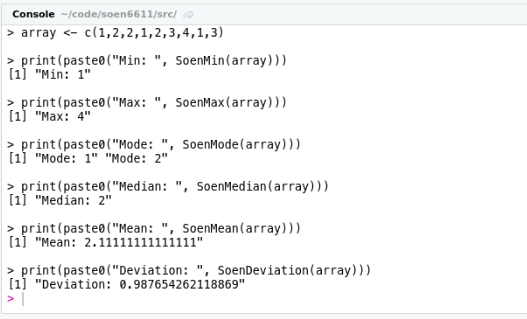
\includegraphics[width=0.7\textwidth]{1.png}
\caption{Results with specified array}
\end{figure}
\begin{figure}[h]
\centering
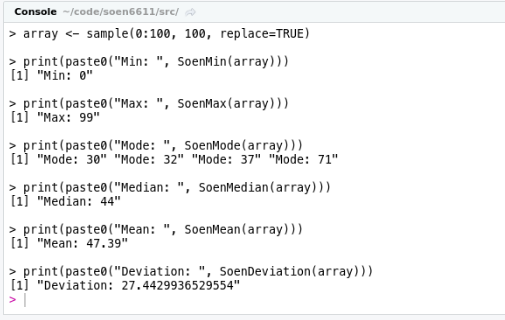
\includegraphics[width=0.7\textwidth]{2.png}
\caption{Results with random array}
\end{figure}
\newpage
\begin{figure}[h]
\centering
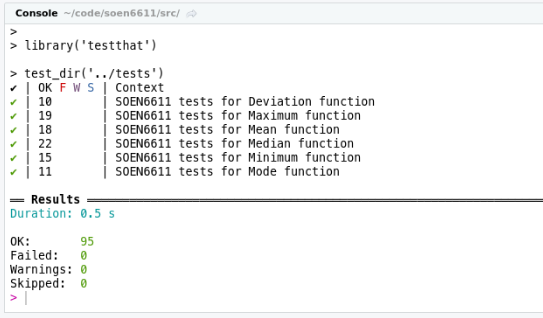
\includegraphics[width=0.7\textwidth]{3.png}
\caption{Tests report}
\end{figure}
\subsubsection{Test initiator}
The main test file for starting all the tests
\begin{lstlisting}[language=R]
library('testthat')

test_dir('../tests')
\end{lstlisting}
\subsubsection{Tests for minimum function}
The set of tests of minimum function.
\begin{lstlisting}[language=R]
context("SOEN6611 tests for Minimum function")

test_that("Positive arrays", {
  expect_that(SoenMin(c(1,2,3,4,5,6)), equals(1))
  expect_that(SoenMin(c(1,2,3,1,1,1)), equals(1))
  expect_that(SoenMin(c(1,1)), equals(1))
  expect_that(SoenMin(c(1)), equals(1))
  expect_that(SoenMin(c(4)), equals(4))
  expect_that(SoenMin(c(5,8,6,7,5,6,9,8,6,5,7,4,7,8,9,6)), equals(4))
  expect_that(SoenMin(c(4,2,3,4,5,1)), equals(1))
})

test_that("Negative arrays", {
  expect_that(SoenMin(c(1,-2,3,-4,5,6)), equals(-4))
  expect_that(SoenMin(c(-1,-2,-3,-1,-1,-1)), equals(-3))
  expect_that(SoenMin(c(-1,-1)), equals(-1))
  expect_that(SoenMin(c(-1)), equals(-1))
  expect_that(SoenMin(c(-6)), equals(-6))
  expect_that(SoenMin(c(-5,8,-6,7,5,-6,9,8,-6,5,7,-4,7,8,9,6)), equals(-6))
  expect_that(SoenMin(c(4,-2,-3,4,5,-1)), equals(-3))
})

test_that("Big arrays", {
  arr <- sample(0:100, 100, replace=TRUE)
  expect_that(SoenMin(arr), equals(min(arr)))
})
\end{lstlisting}

\subsubsection{Tests for Maximum function}
The set of tests of maximum function.
\begin{lstlisting}[language=R]
context("SOEN6611 tests for Maximum function")

test_that("Positive arrays", {
  expect_that(SoenMax(c(1,2,3,4,5,6)), equals(6))
  expect_that(SoenMax(c(1,2,3,1,1,1)), equals(3))
  expect_that(SoenMax(c(5,5,5,5,5,5,5,5,5)), equals(5))
  expect_that(SoenMax(c(1,1)), equals(1))
  expect_that(SoenMax(c(1)), equals(1))
  expect_that(SoenMax(c(8)), equals(8))
  expect_that(SoenMax(c(5,8,6,7,5,6,9,8,6,5,7,4,7,8,9,6)), equals(9))
  expect_that(SoenMax(c(4,2,3,4,5,5)), equals(5))
  expect_that(SoenMax(c(4,2,3,4,3,5)), equals(5))
})

test_that("Negative arrays", {
  expect_that(SoenMax(c(1,-2,3,-4,5,-6)), equals(5))
  expect_that(SoenMax(c(-1,-2,-3,-1,1,-1)), equals(1))
  expect_that(SoenMax(c(-5,-5,-5,-5,-5,-5,-5,-5,-5)), equals(-5))
  expect_that(SoenMax(c(1,-1)), equals(1))
  expect_that(SoenMax(c(-1)), equals(-1))
  expect_that(SoenMax(c(-8)), equals(-8))
  expect_that(SoenMax(c(5,-8,6,-7,5,6,-9,-8,6,5,-7,4,7,-8,-9,6,99)), equals(99))
  expect_that(SoenMax(c(-4,-2,-3,-4,-5,-5)), equals(-2))
  expect_that(SoenMax(c(4,-2,3,-4,3,5)), equals(5))
})

test_that("Big arrays", {
  arr <- sample(0:100, 100, replace=TRUE)
  expect_that(SoenMax(arr), equals(max(arr)))
})
\end{lstlisting}
\subsubsection{Tests for Mode function.}
The set of tests of mode function.
\begin{lstlisting}[language=R]
context("SOEN6611 tests for Mode function")

test_that("Positive arrays", {
  expect_that(SoenMode(c(1,3,4,2,5,4,5)), equals(c(4,5)))
  expect_that(SoenMode(c(1,1,1,2,2,3,4,5,2)), equals(c(1,2)))
  expect_that(SoenMode(c(1,1,1,2,2,3,4,5,2,1)), equals(1))
  expect_that(SoenMode(c(1)), equals(1))
  expect_that(SoenMode(c(5)), equals(5))
})

test_that("Negative arrays", {
  expect_that(SoenMode(c(1,3,-4,2,5,-4,5)), equals(c(-4,5)))
  expect_that(SoenMode(c(-1,1,1,-2,2,3,4,5,2)), equals(c(1,2)))
  expect_that(SoenMode(c(-1,-1,-1,2,2,3,4,5,2,-1)), equals(-1))
  expect_that(SoenMode(c(-1)), equals(-1))
  expect_that(SoenMode(c(-4)), equals(-4))
})

test_that("Big arrays", {
  arr <- sample(0:100, 100, replace=TRUE)
  expect_that(SoenMean(arr), is_a('numeric'))
})
\end{lstlisting}
\subsubsection{Tests for Median function.}
The set of tests of median function.
\begin{lstlisting}[language=R]
context("SOEN6611 tests for Median function")

test_that("Positive arrays even", {
  a1 <- c(1,2,3,2,4,3,2,4,3,2)
  a2 <- c(1,1)
  a3 <- c(9,9)
  a4 <- c(3,2,1,4,3,2,1,3)
  a5 <- c(1,1,1,1,1,1,1,1)
  expect_that(SoenMedian(a1), equals(median(a1)))
  expect_that(SoenMedian(a2), equals(median(a2)))
  expect_that(SoenMedian(a3), equals(median(a3)))
  expect_that(SoenMedian(a4), equals(median(a4)))
  expect_that(SoenMedian(a5), equals(median(a5)))
})

test_that("Positive arrays odd", {
  b1 <- c(1,3,2,6,5,8,3)
  b2 <- c(1)
  b3 <- c(0)
  b4 <- c(1,1,1)
  b5 <- c(1,5,4,5,4,1,1)
  expect_that(SoenMedian(b1), equals(median(b1)))
  expect_that(SoenMedian(b2), equals(median(b2)))
  expect_that(SoenMedian(b3), equals(median(b3)))
  expect_that(SoenMedian(b4), equals(median(b4)))
  expect_that(SoenMedian(b5), equals(median(b5)))
})

test_that("Negative arrays even", {
  c1 <- c(-1,-4,-2,-5,-4,-3)
  c2 <- c(-1,-1)
  c3 <- c(-9,9)
  c4 <- c(-9,-9)
  c5 <- c(-1,-3,2,-2)
  expect_that(SoenMedian(c1), equals(median(c1)))
  expect_that(SoenMedian(c2), equals(median(c2)))
  expect_that(SoenMedian(c3), equals(median(c3)))
  expect_that(SoenMedian(c4), equals(median(c4)))
  expect_that(SoenMedian(c5), equals(median(c5)))
  
})

test_that("Negative arrays odd", {
  d1 <- c(-1,-4,-3,-5,-6,-32,-7)
  d2 <- c(-1,5,6,3,-4,5,-6)
  d3 <- c(-1)
  d4 <- c(-1,-1,-1)
  d5 <- c(-1,1,-1)
  expect_that(SoenMedian(d1), equals(median(d1)))
  expect_that(SoenMedian(d2), equals(median(d2)))
  expect_that(SoenMedian(d3), equals(median(d3)))
  expect_that(SoenMedian(d4), equals(median(d4)))
  expect_that(SoenMedian(d5), equals(median(d5)))
  
})

test_that("Big arrays", {
  arr <- sample(0:100, 100, replace=TRUE)
  expect_that(SoenMedian(arr), equals(median(arr)))
  
  arr2 <- sample(0:4000, 1000, replace=TRUE)
  expect_that(SoenMedian(arr2), equals(median(arr2)))
})
\end{lstlisting}
\subsubsection{Tests for Mean function.}
The set of tests of arithmetic mean function.
\begin{lstlisting}[language=R]
context("SOEN6611 tests for Mean function")

test_that("Positive arrays", {
  expect_that(SoenMean(c(1,2,3,4,5,6)), equals(3.5))
  expect_that(SoenMean(c(1,2,3,1,1,1)), equals(1.5))
  expect_that(SoenMean(c(1,1)), equals(1))
  expect_that(SoenMean(c(1)), equals(1))
  expect_that(SoenMean(c(6)), equals(6))
  expect_that(SoenMean(c(5,8,6,7,5,6,9,8,6,5,7,4,7,8,9,6)), equals(6.625))
  
  a1 <- c(3,5,3,6,7,6,5,3,2,4,3,4,32)
  a2 <- c(0,0,0,0)
  a3 <- c(0)
  a4 <- c(1,0,0,0,0)
  a5 <- c(1,3)
  expect_that(SoenMean(a1), equals(mean(a1)))
  expect_that(SoenMean(a2), equals(mean(a2)))
  expect_that(SoenMean(a3), equals(mean(a3)))
  expect_that(SoenMean(a4), equals(mean(a4)))
  expect_that(SoenMean(a5), equals(mean(a5)))
})

test_that("Negative arrays", {
  a1 <- c(-3,-5,-3,6,-7,6,5,3,-2,4,3,-4,32)
  a2 <- c(-0,-0,-0,-0)
  a3 <- c(-0)
  a4 <- c(-1,-0,-0,-0,-0)
  a5 <- c(1,-3)
  a6 <- c(-3,-5,-3,-7,-2,-4,-5,-3)
  expect_that(SoenMean(a1), equals(mean(a1)))
  expect_that(SoenMean(a2), equals(mean(a2)))
  expect_that(SoenMean(a3), equals(mean(a3)))
  expect_that(SoenMean(a4), equals(mean(a4)))
  expect_that(SoenMean(a5), equals(mean(a5)))
  expect_that(SoenMean(a6), equals(mean(a6)))
})

test_that("Big arrays", {
  arr <- sample(0:100, 100, replace=TRUE)
  expect_that(SoenMean(arr), equals(mean(arr)))
})
\end{lstlisting}
\subsubsection{Tests for Deviation function.}
The set of tests of deviation function.
\begin{lstlisting}[language=R]
context("SOEN6611 tests for Deviation function")

test_that("Positive arrays", {
  a1 <- c(1,4,5,3,1,5,4)
  a2 <- c(1,1)
  a3 <- c(13,5,2,3,21,3,2)
  a4 <- c(1,1,1,1,1)
  expect_that(SoenDeviation(a1), equals(sd(a1)*(sqrt((length(a1)-1)/length(a1)))))
  expect_that(SoenDeviation(a2), equals(sd(a2)*(sqrt((length(a2)-1)/length(a2)))))
  expect_that(SoenDeviation(a3), equals(sd(a3)*(sqrt((length(a3)-1)/length(a3)))))
  expect_that(SoenDeviation(a4), equals(sd(a4)*(sqrt((length(a4)-1)/length(a4)))))
})

test_that("Negative arrays", {
  c1 <- c(1,-4,3,-2,-4)
  c2 <- c(-1,-1)
  c3 <- c(-1,-1,-1,-1)
  c4 <- c(-1,3,-12,4,-1)
  expect_that(SoenDeviation(c1), equals(sd(c1)*(sqrt((length(c1)-1)/length(c1)))))
  expect_that(SoenDeviation(c2), equals(sd(c2)*(sqrt((length(c2)-1)/length(c2)))))
  expect_that(SoenDeviation(c3), equals(sd(c3)*(sqrt((length(c3)-1)/length(c3)))))
  expect_that(SoenDeviation(c4), equals(sd(c4)*(sqrt((length(c4)-1)/length(c4)))))
  
})

test_that("Big arrays", {
  arr <- sample(0:100, 100, replace=TRUE)
  expect_that(SoenDeviation(arr), equals(sd(arr)*(sqrt((length(arr)-1)/length(arr)))))

  arr2 <- sample(0:4000, 1000, replace=TRUE)
  expect_that(SoenDeviation(arr2), equals(sd(arr2)*(sqrt((length(arr2)-1)/length(arr2)))))
})
\end{lstlisting}

%-----------------------------------------------------------------
\section{Part - Cyclomatic complexity}
Cyclomatic complexity is a software metric used to measure the complexity of a program. These metric, measures independent paths through program source code. Cyclomatic complexity can be calculated with respect to functions, modules, methods or classes within a program.
\begin{equation}
    \textbf{Complexity of the Program V(G)} = E - N + 2
\end{equation}
Where, E - Number of edges, N - Number of Nodes in the Flow graph.
\begin{equation}
    \textbf{Complexity of the Program V(G)} = P + 1 
\end{equation}
Where P = Number of node that contains condition.\cite{CN}
\begin{table}[h]
\centering
\begin{tabular}{|l|l|l|}
\hline
\multicolumn{1}{|c|}{\textbf{File}} & \multicolumn{1}{c|}{\textbf{Function}} & \multicolumn{1}{c|}{\textbf{Cyclomatic number}} \\ \hline
init.R & Flow of calls & 1 \\ \hline
min.R & SoenMin() & 5 \\ \hline
max.R & SoenMax() & 5 \\ \hline
mode.R & SoenMode() & 9 \\ \hline
median.R & SoenMedian() & 4 \\ \hline
mean.R & SoenMean() & 4 \\ \hline
deviation.R & SoenDeviation() & 4 \\ \hline
\multirow{4}{*}{stdlib.R} & SoenLen() & 2 \\ \cline{2-3} 
 & SoenSqrtA() & 5 \\ \cline{2-3} 
 & SoenSqrtB() & 4 \\ \cline{2-3} 
 & SoenSort() & 2 \\ \hline
\textbf{Total} & \textbf{} & \textbf{45} \\ \hline
\end{tabular}
\caption{Cyclomatic complexity.}
\label{my-label}
\end{table}

The \textbf{Cyclomatic Number} for the descriptive-statistic project is \textbf{45}.\\

\textbf{Conclusion}: According to the Range-Risk distribution of complexity number. Each file in the project has a \textbf{simple} control flow, less than 10. But the whole project has cyclomatic number equal 45, that falls under category of High risk assessment. The source code has a very "complex", but manageable, control flow. 
%-----------------------------------------------------------------
\newpage
\section{Part - Object-oriented metrics}
\begin{figure}[h]
\centering
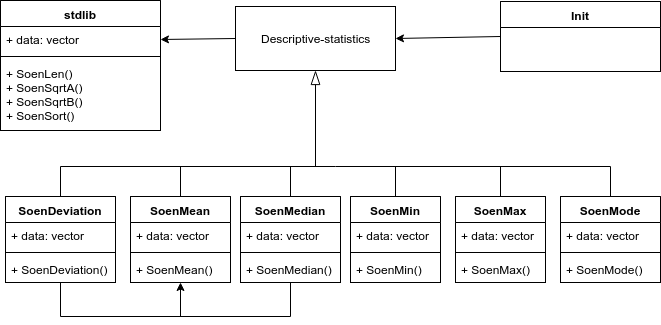
\includegraphics[width=\textwidth]{classdiagram.png}
\caption{Class diagram}
\end{figure}
\subsection{Weighted Methods per Class}

\begin{table}[h]
\centering
\begin{tabular}{|l|l|l|}
\hline
\multicolumn{1}{|c|}{\textbf{Class}} & \multicolumn{1}{c|}{\textbf{Method}} & \multicolumn{1}{c|}{\textbf{Weight}} \\ \hline
init.R & Flow of calls & 1 \\ \hline
min.R & SoenMin() & 5 \\ \hline
max.R & SoenMax() & 5 \\ \hline
mode.R & SoenMode() & 9 \\ \hline
median.R & SoenMedian() & 4 \\ \hline
mean.R & SoenMean() & 4 \\ \hline
deviation.R & SoenDeviation() & 4 \\ \hline
\multirow{4}{*}{stdlib.R} & SoenLen() & 2 \\ \cline{2-3} 
 & SoenSqrtA() & 5 \\ \cline{2-3} 
 & SoenSqrtB() & 4 \\ \cline{2-3} 
 & SoenSort() & 2 \\ \hline
\end{tabular}
\caption{WMC.}
\end{table}
\begin{equation}
    \textbf{WMC} =\sum^{n}_{i=1}{c_{i}(M_{i})}  
\end{equation}
Where C a class with methods M1 to Mn. Let c1(M1), to cn(Mn) be the complexity (weights) of the methods \cite{OOD}
\begin{equation}
    \textbf{WMC} = 1+5+5+9+4+4+4+2+5+4+2 = 45  
\end{equation}
\subsection{Coupling Factor}

The coupling factor (CF) measures the average coupling between classes. 
\begin{equation}
    \textbf{CF} =\frac{\sum^{n}_{i=1}{\Bigg[\sum^{n}_{j=1}{isClient(C_{i},C_{j})\Bigg]}}}{n^2-n}  
\end{equation}
\begin{equation}
    \textbf{CF} =\frac{0+6+2+1+2+1+1+1}{8^2-8}  
\end{equation}
\begin{equation}
    \textbf{CF} = 0.25
\end{equation}
The Coupling Factor is equal to 0.25.
\subsection{Lack of Cohesion in Methods}
The Lack of Cohesion in methods (LCOM).
\begin{equation}
    \textbf{LCOM} =\frac{\frac{1}{a}\Big[\sum^{a}_{i=1}{\mu(A_{i})\big]-m}}{1-m}
\end{equation}

\begin{equation}
    LCOM_{stdlib} =\frac{\frac{1}{2}\times[2+2]-4}{1-4} = \frac{2}{3}
\end{equation}
\begin{equation}
    LCOM_{min} = \frac{\frac{1}{1}\times1-1}{1-1} = \frac{0}{0} = 0
\end{equation}
\begin{equation}
    LCOM_{max} = \frac{\frac{1}{1}\times1-1}{1-1} = \frac{0}{0} = 0
\end{equation}
\begin{equation}
    LCOM_{mode} = \frac{\frac{1}{1}\times1-1}{1-1} = \frac{0}{0} = 0
\end{equation}
\begin{equation}
    LCOM_{median} = \frac{\frac{1}{1}\times1-1}{1-1} = \frac{0}{0} = 0
\end{equation}
\begin{equation}
    LCOM_{mean} = \frac{\frac{1}{1}\times1-1}{1-1} = \frac{0}{0} = 0
\end{equation}
\begin{equation}
    LCOM_{deviation} = \frac{\frac{1}{1}\times1-1}{1-1} = \frac{0}{0} = 0
\end{equation}

For six classes LCOM is 0 and that means that these classes have maximum cohesion. Class stdlib has LCOM = $\frac{2}{3}$ and that means that cohesion in this class is not high, but not too low.
%-----------------------------------------------------------------
\section{Part - SLOC}
The most common definition of physical SLOC is a count of lines of source code excluding comment lines.
So, manually our \textbf{Physical SLOC = 265}. The Logical SLOC is number of executable "statements", such as if, for, while, <- and other expressions that may affect on the execution, excluding the comments and useless lines such closing bracket. So, manually our \textbf{Logical SLOC = 234}.\\

\textbf{Physycal SLOC = 265} and \textbf{Logical SLOC = 236} according to the GitHub code editor as a tool for calculating the SLOC.
%-----------------------------------------------------------------
\section{Part - Correlations}
\subsection{Scatter plot}
\begin{table}[h]
\centering
\begin{tabular}{|l|l|l|}
\hline
\multicolumn{1}{|c|}{\textbf{Class}} & \multicolumn{1}{c|}{\textbf{WMC}} & \textbf{Logical SLOC} \\ \hline
init & 1 & 25 \\ \hline
min & 5 & 21 \\ \hline
max & 5 & 21 \\ \hline
mode & 9 & 39 \\ \hline
median & 4 & 23 \\ \hline
mean & 4 & 20 \\ \hline
deviation & 4 & 23 \\ \hline
stdlib & 13 & 64 \\ \hline
\end{tabular}
\caption{WMC and LSLOC for each class.}
\end{table}

\begin{figure}[h]
\centering
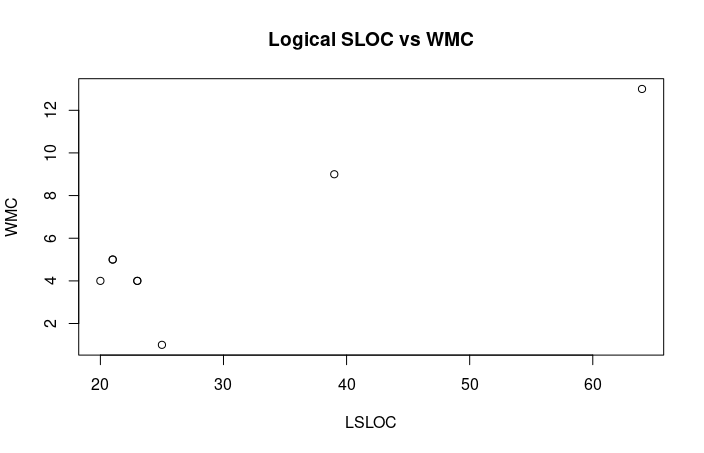
\includegraphics[width=\textwidth]{Rplot.png}
\caption{Scatter Plot}
\end{figure}

\subsection{Correlation coefficient}
Since the attributes are no distributed normally we can apply the Spearman's Rank Correlation Coefficient $r_{s}$.\cite{Correlation}
\begin{equation}
    r_{s} = 1-\frac{6\times\sum^{n}_{i=1}{d_{i}^2}}{n^3-n}  
\end{equation}

\begin{table}[h]
\centering
\begin{tabular}{|l|l|l|l|l|l|l|}
\hline
\multicolumn{1}{|c|}{\textbf{Class}} & \multicolumn{1}{c|}{\textbf{WMC$(x_{i})$}} & \textbf{Rank$(x_{i})$} & \textbf{Logical SLOC$(y_{i})$} & \textbf{Rank$(y_{i})$} & \textbf{d} & \textbf{$d^2$}\\ \hline
init      & 1  & 1   & 25 & 6   & -5 & 25\\ \hline
min       & 5  & 5.5 & 21 & 2.5 & 3.5 & 12.25\\ \hline
max       & 5  & 5.5 & 21 & 2.5 & 3.5 & 12.25\\ \hline
mode      & 9  & 7   & 39 & 7   & 0 & 0\\ \hline
median    & 4  & 3   & 23 & 4.5 & -1.5 & 2.25\\ \hline
mean      & 4  & 3   & 20 & 1   & 2 & 4\\ \hline
deviation & 4  & 3   & 23 & 4.5 &  -1.5 & 2.25\\ \hline
stdlib    & 13 & 8   & 64 & 8   &  0 & 0\\ \hline
\end{tabular}
\caption{Data for Spearman's correlation coefficient}
\end{table}

\begin{equation}
    r_{s} = 1-\frac{6\times(25+12.25+12.25+0+2.25+4+2.25+0)}{8^3-8}  
\end{equation}
\begin{equation}
    r_{s} = 1-\frac{348}{504}  
\end{equation}\\
\begin{equation}
    r_{s} = 0.31  
\end{equation}
We have a positive correlation between WMC and Logilal SLOC for classes.
%-----------------------------------------------------------------
\newpage
\section{Part - Glossary}
\begin{table}[h]
\centering
\begin{tabular}{|l|l|}
\hline
\multicolumn{1}{|c|}{\textbf{Term}} & \multicolumn{1}{c|}{\textbf{Definition}} \\ \hline
GQM & Goal Question Metric \\ \hline
UCM & Use Case Model \\ \hline
UCP & Use Case Points \\ \hline
UUCP & Unadjusted Use Case Points \\ \hline
UUCW & Unadjusted Use Case Weight \\ \hline
UAW & Unadjusted Actor Weight \\ \hline
TCF & Technical Complexity Factor \\ \hline
ECF & Environment Complexity Factor \\ \hline
PF & Productivity Factor \\ \hline
COCOMO & Constructive Cost Model \\ \hline
Cyclomatic number & Indicator of internal complexity \\ \hline
WMC & Weighted Method per Classes \\ \hline
CF & Coupling Factor \\ \hline
LCOM & Lack of Cohesion in Methods \\ \hline
SLOC & Source Line Of Code \\ \hline
$r_{s}$ & Spearman Rank Correlation Coefficient \\ \hline
\end{tabular}
\caption{Glossary}
\end{table}
%-----------------------------------------------------------------
%Don't delete below
\bibliography{ref}{}
\bibliographystyle{unsrt}
\end{document}